\documentclass[11pt]{article}
\usepackage{xcolor}
\usepackage{pgfplots}
\usepackage[T1]{fontenc}
\usepackage[utf8]{inputenc}
\usepackage{xcolor}
\usepackage{pgfplots}
\usepackage{colortbl}
\usepackage{pgfplots}
\usepackage[T1]{fontenc}
\usepackage[utf8]{inputenc}
\usepackage{xcolor}

\begin{document}

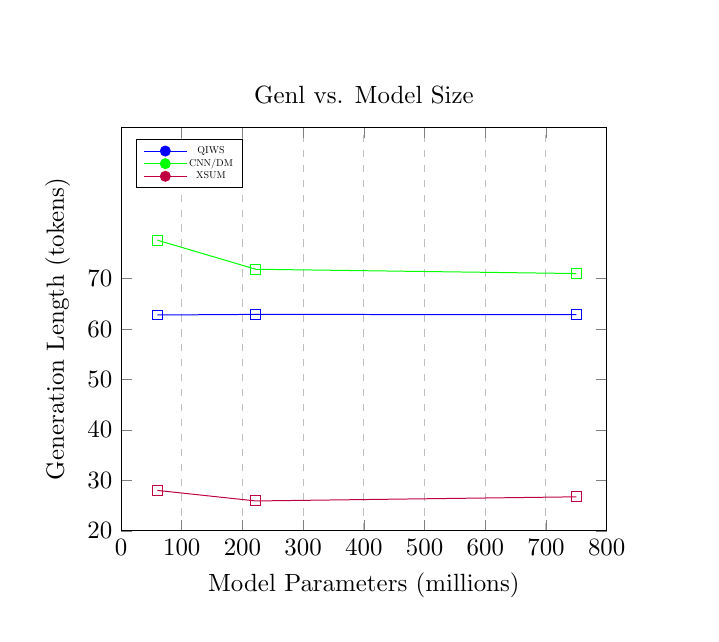
\begin{tikzpicture}
\scalebox{0.9}{
\begin{axis}[
    title={Genl vs. Model Size},
    ylabel={Generation Length (tokens)},
    xlabel={Model Parameters (millions)},
    ymin=20, ymax=100,
    xmin=0, xmax=800,
    ytick={20,30,40,50,60,70},
    xtick={0,100,200,300,400,500,600,700,800},
    legend pos=north west,
    xmajorgrids=true,
    grid style=dashed,
    legend style={nodes={scale=0.4, transform shape}}, 
    legend image post style={mark=*}
]
\addplot[
    color=blue,
    mark=square,
    ]
    coordinates {
    (60,62.79) ( 222,62.91) (750,62.85) 
    };
\addplot[
    color=green,
    mark=square,
    ]
    coordinates {
    (60, 77.62) (222, 71.86) (750,71.01)
    };  
\addplot[
    color=purple,
    mark=square,
    ]
    coordinates {
    (60,28.01) (222, 25.92) (750,26.74)
    };
\legend{QIWS, CNN/DM , XSUM}
 \end{axis}}
\end{tikzpicture}

\end{document}